\chapter{基于累加器的FIR滤波器设计}
\begin{introduction}
  \item \textit{使用Simulink进行FIR滤波器的仿真;}
  \item \textit{MATLAB绘制FIR滤波器的输入输出响应;}
  \item \textit{Verilog编写简单的FIR滤波器;}
  \item \textit{基于累加器的FIR滤波器的FPGA实现。}
\end{introduction}
\section{实验背景与目的}
随着 FPGA(Field Programmable Gate Array)技术的广泛应用,数字信号处理(DSP)在通信、音频处理和工业控制等领域的需求不断增长。FIR(有限脉冲响应)滤波器作为一种重要的数字滤波技术,以其线性相位特性和稳定性,在硬件实现中占据重要地位。

在 FPGA 设计中,乘法-累加(MAC)运算是 FIR 滤波器的核心计算过程,而累加器结构能够高效执行这一运算,提高计算吞吐量和资源利用率。本实验围绕 FIR 滤波器的硬件实现,重点研究基于累加器的FIR滤波器实现方法,并结合 MATLAB 和 Simulink 进行算法仿真,以验证滤波器性能。另外,通过本实验,还可以进一步熟悉Vivado IP核的调用方法。

\section{实验原理}

\subsection{FIR 滤波器}

有限脉冲响应(Finite Impulse Response, FIR)滤波器是一种线性时不变系统,其输出仅依赖于当前及有限个历史输入样本,而不会受到过去输出的影响。其数学表达式为:

\begin{equation}
    y[n] = \sum_{k=0}^{N-1} h[k] x[n-k]
\end{equation}

其中:
\begin{itemize}
    \item $x[n]$ 为输入信号,
    \item $y[n]$ 为输出信号,
    \item $h[k]$ 为滤波器系数(即脉冲响应),
    \item $N$ 为滤波器的阶数。
\end{itemize}

FIR 滤波器的一个重要特点是其\textbf{线性相位特性},即滤波器系数满足对称性:

\begin{equation}
    h[k] = \pm h[N-1-k], \quad k = 0,1,\dots, N-1
\end{equation}

这种特性保证了不同频率分量不会产生相位失真,在许多信号处理应用中至关重要。

\subsection{FIR 滤波器的结构}

FIR 滤波器的实现主要基于乘积求和,可以采用直接型(横截型)、线性相位型和频率采样型等结构。最容易实现的是直接型结构。


直接型 FIR 滤波器的基本组成部分包括:
\begin{itemize}
    \item 延迟单元(Delay Elements):用于存储输入数据 $x[n]$ 的历史值,通常使用移位寄存器实现。
    \item 乘法器(Multipliers):将输入信号的延迟版本与滤波器系数 $h[k]$ 相乘。
    \item 加法器(Adders):对所有乘积求和,生成最终的滤波器输出。
\end{itemize}

在 FPGA 设计中,FIR 滤波器可以通过 乘法-累加(MAC, Multiply-Accumulate) 结构优化计算效率,同时利用 DSP 资源 进行并行计算,提高吞吐量。此外,为了减少乘法运算,通常采用系数量化和移位累加(Shift-and-Add)技术。

本实验将基于 FPGA 设计一个 FIR 滤波器,并采用累加器结构进行优化,以提高计算性能和资源利用率。
\section{实验使用软件/平台}
\begin{itemize}
  \item Xilinx Vivado 2024.2;\footnote{笔者在这次实验时将Vivado部署到了Linux中,Implementation的速度远高于Windows,且官网可以下载到免费的版本。配置的过程见本章结尾。}
  \item eNodeX 30B软件无线电创新平台;
  \item 示波器。
  \item MATLAB \& Simulink R2024b;
\end{itemize}
\section{实验内容}
\subsection{FIR滤波器的Simulink仿真}
为了直观描述FIR数字滤波器的结构,使用Simulink搭建两种结构的FIR数字滤波器。其中第二种并不常见,且实现起来无法复用延时器,故仅作仿真用。

\begin{figure}[htbp]
  \subfloat[横截型FIR滤波器\label{subfig:hengjie}]{\includegraphics[width = 0.45\textwidth]{figure/exp4/circuit_exp4.png}}
  \hfill
  \subfloat[FIR滤波器]{\includegraphics[width = 0.45\textwidth]{figure/exp4/circuit_exp4_2.png}}
  \caption{两种FIR滤波器的结构}
  \label{fig:exp4:simulink}
\end{figure}
搭建两种结构的数字滤波器如图~\ref{fig:exp4:simulink}。图~\ref{subfig:hengjie}~是典型的横截型滤波器结构,输入为1MHz和10MHz的两股正弦信号经过加法器后通过该滤波器输出。滤波器由四个延时器和一个加法器组成,这在模型中也直观地体现出来了。第二种结构采用了四种不同的延时器,分别延时1、2、3、4个单位时钟,这让我们清楚地推出FIR滤波器的系统函数:
\begin{equation}\label{eqn:fir}
  H(z) = 1 + z^{-1} + z^{-2} +z^{-3} +z^{-4}
\end{equation}
令$z = e^{j\omega}$,可得系统的频率响应,显然可以看出该滤波器是一个低通滤波器。

启动仿真,观察滤波前和滤波后的时域波形如图~\ref{fig:exp4:scope}。可以看到,滤波前信号含有大量高频杂波,而滤波后信号变平滑。滤波后信号有约5倍的增益,这可以从公式~\ref{eqn:fir}~中找到原因。

\begin{figure}[htbp]
  \centering
  \includegraphics[width = 0.75\textwidth]{figure/exp4/scope.pdf}
  \caption{滤波前(橙)和滤波后(蓝)的时域波形}
  \label{fig:exp4:scope}  
\end{figure}

接下来进行频谱分析(图~\ref{fig:exp4:spectrum}~)。可以看出滤波前信号在1M和10M处包含峰值,这符合加和信号的特征;滤波后,高频分量被滤除,而低频分量出现一定失真。

\begin{figure}[htbp]
  \centering
  \subfloat[滤波前信号频谱]{\includegraphics[width = 0.45\textwidth]{figure/exp4/input.png}}
  \hfill
  \subfloat[滤波后信号频谱]{\includegraphics[width = 0.45\textwidth]{figure/exp4/output.png}}
  \caption{信号频谱分析}
  \label{fig:exp4:spectrum}
\end{figure}

\begin{remark}
两种形式的滤波器仿真结果相同,此处不再展示第二种滤波器的仿真结果。
\end{remark}

\subsection{FIR滤波器的MATLAB仿真}
编写MATLAB代码如下:
\begin{lstlisting}[language=matlab]
f1=1e7;
f2=1e6;
fs=5e7;
t=0:1/fs:0.00005;

s=sin(2*pi*f1*t)+sin(2*pi*f2*t); %产生两个频率信号的叠加信号
b=[1,1,1,1,1];
y=filter(b,1,s);
%累加器(滤波器)的系数
%求出滤波器输出序列

%第1张图绘制输入输出信号
figure(1);
subplot(211); plot(t,s);
legend('输入信号波形');
xlabel('时间(s)');ylabel('幅度(v)');
subplot(212);plot(t,y);
legend('输出信号波形');
xlabel('时间(s)');ylabel('幅度(v)');
%第2张图绘制滤波器频率响应
figure(2);
freqz(b,1)
\end{lstlisting}
运行代码,可得到输入输出信号的波形,以及滤波器的频率响应如图~\ref{fig:exp4:matlab}。
\begin{figure}[htbp]
  \centering
  \subfloat[滤波前后信号波形]{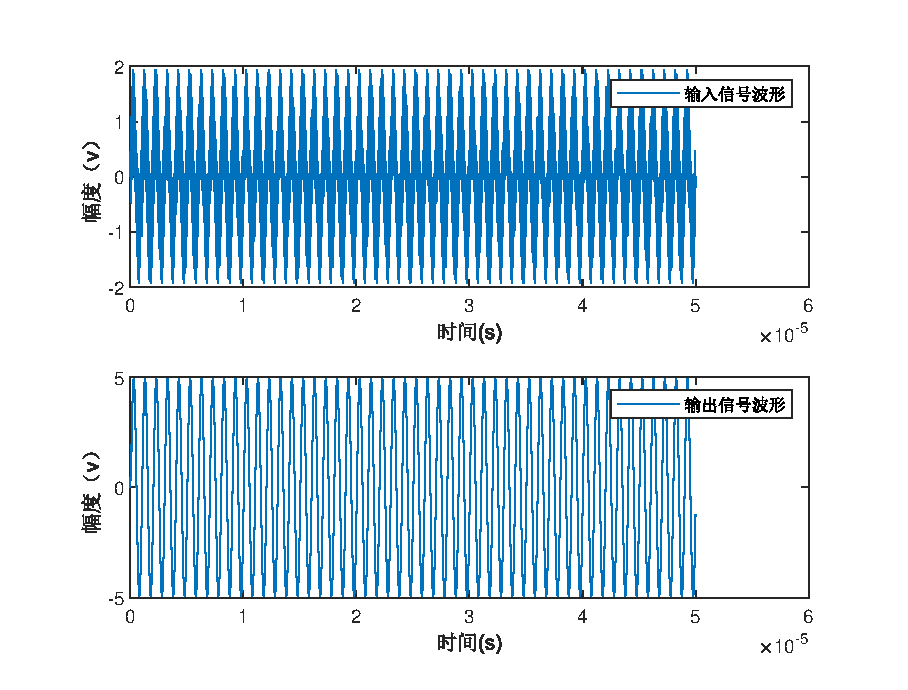
\includegraphics[width = 0.45\textwidth]{figure/exp4/fig1.eps}}
  \hfill
  \subfloat[滤波器的频率响应]{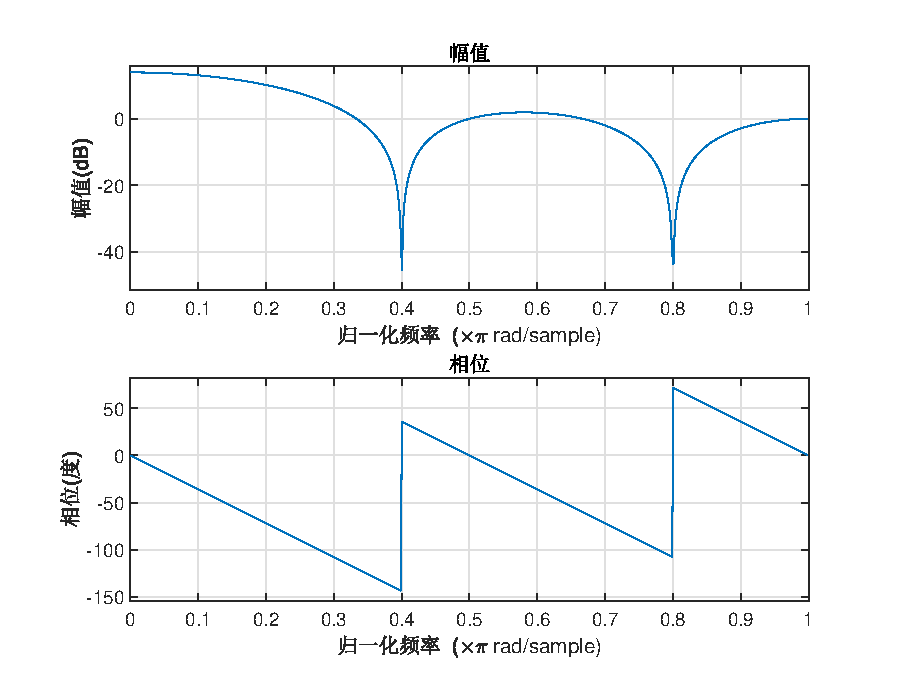
\includegraphics[width = 0.45\textwidth]{figure/exp4/fig2.eps}}
  \caption{信号频谱分析}
  \label{fig:exp4:matlab}
\end{figure}
\subsection{基于累加器的FIR滤波器的FPGA实现}
基于公式~\ref{eqn:fir}~和图~\ref{subfig:hengjie},可以设计一个基于累加器的FIR滤波器。需要注意的是,由于输出为五个输入相加,故输出的最大可能位宽为输入位宽+4。FIR滤波器的输入输出端口如表~\ref{table:interface_fir}~所示。

\begin{table}[htbp]
  \centering
  \begin{tabular}{ccc}
    \toprule
     信号名 & 意义 & 端口类型\\
    \midrule
      \texttt{clk} & 50MHz时钟信号 & Input \\
     \texttt{xin} & 10-bit 加和后量化正弦信号 & Input \\
     \texttt{yout} & 14-bit 滤波后量化信号输出 & Output \\
    \bottomrule
  \end{tabular}
  \caption{FIR模块接口说明}
  \label{table:interface_fir}
\end{table}

下面是该模块的代码,可见输入数据通过4个寄存器后生成四个时刻的数据,再相加得到滤波器的输出。
\begin{lstlisting}[language=verilog,caption={FIR滤波器模块}]
module FIR(
      input clk,                      // 50MHz Clock
      input signed [10:0] xin,        // input
      output signed [13:0] yout       // output
  );
  
  reg signed [10:0] x1,x2,x3,x4; // cascaded registers
  always @(posedge clk) begin
  x1 <= xin; 
  x2 <= x1; 
  x3 <= x2; 
  x4 <= x3;
  end
  
  // Output
  assign yout =xin + x1 + x2 + x3 + x4; 
  endmodule
  \end{lstlisting}
\begin{lstlisting}[language=verilog, caption={Testbench文件}]
  `timescale 1ns / 1ps

  module tb_FIR;
  
  reg clk;    // 100MHz
  reg clk_DAC1, clk_DAC2, wrt_DAC1, wrt_DAC2;
  reg mode_DAC;
  reg [13:0] filter_input;
  reg [13:0] filter_output;
  
  
  TOP module_top(
  .PL_CLK_100MHz(clk), 
  .LS_DAC2_DB(filter_output),
  .LS_DAC2_CLK(clk_DAC2),
  .LS_DAC2_WRT(wrt_DAC2),
  .LS_DAC1_DB(filter_input),
  .LS_DAC1_CLK(clk_DAC1),
  .LS_DAC1_WRT(wrt_DAC1),
  .LS_DAC_MODE(mode_DAC)
  );
  
  //clock
  initial begin
  clk = 0; 
  end 
  always #5 clk <= !clk;    
  
  initial begin
      $dumpfile("fir.vcd");
      $dumpvars(0, tb_FIR);
  end
  
  initial begin
  #1000000 $stop(2);
  end
  
  endmodule
  
\end{lstlisting}

基于此模块设计,编写测试模块(Testbench)如下。在测试模块中调用\textit{DDS Compiler} IP核生成1MHz和10MHz的正弦信号并相加后,对FIR模块进行测试。
\begin{lstlisting}[language=verilog, caption={Testbench文件}]
  `timescale 1ns / 1ps
  module tb_FIR;
  
    reg clk;
    wire signed [10:0] xin;  // FIR Input
    wire signed [13:0] yout;  // FIR Output
    wire signed [9:0] sin1M, sin10M;  // Generated by DDS
  
  
    FIR DUT (
        .clk (clk),
        .xin (xin),
        .yout(yout)
    );
  
    // Generate 50MHz Clock signal for testbench
    initial begin
      clk = 0;
    end
  
    always #10 clk <= ~clk;
    
    SIN_1M sin_1M (
        .aclk                (clk),      // input wire aclk
        .s_axis_config_tvalid(1'b1),     // input wire s_axis_config_tvalid
        .s_axis_config_tdata (16'H51E),  // input wire [15 : 0] s_axis_config_tdata
        .m_axis_data_tvalid  (),         // output wire m_axis_data_tvalid
        .m_axis_data_tdata   (sin1M)     // output wire [15 : 0] m_axis_data_tdata
    );
    SIN_10M sin_10M (
        .aclk                (clk),       // input wire aclk
        .s_axis_config_tvalid(1'b1),      // input wire s_axis_config_tvalid
        .s_axis_config_tdata (16'H3333),  // input wire [15 : 0] s_axis_config_tdata
        .m_axis_data_tvalid  (),          // output wire m_axis_data_tvalid
        .m_axis_data_tdata   (sin10M)     // output wire [15 : 0] m_axis_data_tdata
    );
    // Assignments
    assign xin = sin1M + sin10M;
  endmodule
  
\end{lstlisting}

测试结果如图~\ref{fig:exp4:result}~所示。\footnote{需要在xsim中调整数据格式(Radix)为Signed Decimal,波形格式为Analog。}可以看出设计的FIR滤波器成功滤除了高频的10MHz信号,而保留了1MHz的信号,这符合低通滤波器的特性。
\begin{figure}[htbp]
  \centering
  \includegraphics[width=0.75\textwidth]{figure/exp4/vivado_waveform.png}
  \caption{FIR滤波器滤波结果}
  \label{fig:exp4:result}
\end{figure}

为了进一步验证该模块的可靠性,将设计部署到FPGA上。在FIR模块之上,完成一个顶层模块,接口为FPGA(Zynq-7000)约束文件中的DAC接口。需要注意的是,该FPGA的时钟主频为100MHz,故需要调用\textit{Clocking Wizard}生成一个50MHz的时钟。该FPGA有两路DAC,故只能选择两路信号最终显示到示波器上,笔者选择滤波前和滤波后的两个信号。由于DAC的输出位宽为14,故对于不满14位的输入数据,按照二进制补码规则向上补齐符号位至14位。\footnote{在模拟域下,相当于幅度缩小16倍,但相对幅度是不变的。}代码如下。

\begin{lstlisting}[language=verilog,caption={顶层模块}]
  module TOP (
    PL_CLK_100MHz,
    LS_DAC2_DB,
    LS_DAC2_CLK,
    LS_DAC2_WRT,
    LS_DAC1_DB,
    LS_DAC1_CLK,
    LS_DAC1_WRT,
    LS_DAC_MODE
);
  // Inputs and Outputs
  input wire PL_CLK_100MHz;
  // board clock frequency = 100MHz, need to be written in tb


  // DAC Parameters
  output signed [13:0] LS_DAC2_DB;
  output LS_DAC2_CLK;
  output LS_DAC2_WRT;
  output signed [13:0] LS_DAC1_DB;
  output LS_DAC1_CLK;
  output LS_DAC1_WRT;
  output LS_DAC_MODE;


  wire clk;
  wire signed [13:0] fir_out;
  wire signed [9:0] sin_1M;
  wire signed [9:0] sin_10M;
  wire signed [10:0] sum;
  wire signed [13:0] sum_ext;
//   wire [15:0] sin_1M_temp;
//   wire [15:0] sin_10M_temp;

  // Clock IP: Generate 50MHz synchrous clk 
  CLK_50M module_clk_50M (
      // Clock out ports
      .clk_out1(clk),           // output clk_out1
      // Status and control signals
      .locked  (),              // output locked
      // Clock in ports
      .clk_in1 (PL_CLK_100MHz)  // input clk
  );



  SIN_1M module_sin_1M (
      .aclk                (clk),      // input wire aclk
      .s_axis_config_tvalid(1'b1),     // input wire s_axis_config_tvalid
      .s_axis_config_tdata (16'H51E),  // input wire [23 : 0] s_axis_config_tdata
      .m_axis_data_tvalid  (),         // output wire m_axis_data_tvalid
      .m_axis_data_tdata   (sin_1M)    // output wire [15 : 0] m_axis_data_tdata
  );

  SIN_10M module_sin_10M (
      .aclk                (clk),       // input wire aclk
      .s_axis_config_tvalid(1'b1),      // input wire s_axis_config_tvalid
      .s_axis_config_tdata (16'H3333),  // input wire [15 : 0] s_axis_config_tdata
      .m_axis_data_tvalid  (),          // output wire m_axis_data_tvalid
      .m_axis_data_tdata   (sin_10M)    // output wire [15 : 0] m_axis_data_tdata
  );

  FIR module_fir (
      .clk (clk),
      .xin (sum),     // 10 bits
      .yout(fir_out)  // 14 bits
  );

  // ILA Probe
  ILA module_probe (
      .clk(clk),  // input wire clk
      .probe0(sum_ext),  // 14 bits 
      .probe1(fir_out)  // 14 bits
  );


  // assignments

  assign sum         = sin_1M + sin_10M;  // auto truncate
  assign sum_ext     = {{3{sum[10]}}, sum};  // fill to 14 bits for output
//   assign sin_1M      = sin_1M_temp[15:6];
//   assign sin_10M     = sin_10M_temp[15:6];  // truncate only

  // DAC OUTPUT

  assign LS_DAC_MODE = 1'b1;
  assign LS_DAC1_DB  = sum_ext + 14'h2000;  // to unsigned data
  assign LS_DAC1_CLK = !clk;
  assign LS_DAC1_WRT = LS_DAC1_CLK;
  assign LS_DAC2_DB  = fir_out + 14'h2000;  // to unsigned data
  assign LS_DAC2_CLK = clk;
  assign LS_DAC2_WRT = LS_DAC2_CLK;

endmodule

\end{lstlisting}

生成TOP模块的比特流,并烧录到FPGA开发板上,可从ILA和示波器出看到波形(图~\ref{fig:exp4:Implementation})。
\begin{figure}[htbp]
  \centering
  \subfloat[滤波前(上)与滤波后(下)的ILA波形]{\includegraphics[width = 0.95\textwidth]{figure/exp4/waveform_ila.png}}
  \newline
  \subfloat[滤波前(黄色)与滤波后(绿色)的示波器波形]{\includegraphics[width = 0.95\textwidth]{figure/exp4/waveform.jpg}}
  \caption{FPGA中滤波器输入输出的ILA与示波器波形}
  \label{fig:exp4:Implementation}
\end{figure}

\section{思考与讨论}
\subsection{更改参数的FIR滤波器实现}
更改FIR滤波器模块,使其适配公式~\ref{eqn:fir2}~的滤波器设置。
\begin{equation}\label{eqn:fir2}
  H(z) = 1 + 3z^{-1} + 2z^{-2} + 3z^{-3} + 2z^{-4} + 2.5z^{-5}
\end{equation}

注意到滤波器系数出现了小数,可以使用向右移位1位的方式构建0.5倍数。Verilog代码如下:
\begin{lstlisting}[language=verilog,caption={新版滤波器模块}]
module FIR_NEW (
    input                clk,  // 50MHz Clock
    input  signed [10:0] xin,  // input
    output signed [13:0] yout  // output
);

  reg signed [11:0] x1, x2, x3, x4, x5;  // cascaded registers
  always @(posedge clk) begin
    x1 <= xin;
    x2 <= x1;
    x3 <= x2;
    x4 <= x3;
    x5 <= x4;
  end

  // Output
  assign yout = xin + 3 * x1 + (x2 << 1) + 3 * x3 + (x4 << 1) + (x5 << 1) + (x5 >> 1);
endmodule

\end{lstlisting}

使用Testbench模块进行仿真,得到波形如图~\ref{fig:exp4:result2}。可以看到,波形相较均值滤波器,高频分量并未完全滤除。
\begin{figure}[htbp]
  \centering
  \includegraphics[width=0.75\textwidth]{figure/exp4/vivado_waveform_2.png}
  \caption{新版FIR滤波器滤波结果}
  \label{fig:exp4:result2}
\end{figure}

这是因为新版滤波器在高频下依然拥有比均值滤波器更高的频率响应(系数全正),导致高频分量与低频分量的差距减小。
\subsection{Linux系统下的 Vivado 配置}
FPGA的开发套件来源于芯片设计的开发套件,而绝大部分的芯片设计软件部署在Linux上。由此,Vivado作为典型的FPGA开发套件,可能也支持(甚至更适配)Linux开发环境。查阅资料可知,Vivado的Windows发行版(2021年)仍存在编译速度慢、工程代码同步、log打印占用时间/资源多等缺陷。因此,笔者将Vivado部署在Linux环境中后,完成了这次实验。安装的过程大量参考了\url{https://blog.csdn.net/weixin_46423500/article/details/142331804},将其重述如下。

使用Ubuntu24.04 Linux发行版进行环境配置。首先安装依赖:
\begin{lstlisting}[language=bash]
  sudo apt-get update
  sudo apt-get upgrade
  sudo apt-get install libncurses5
  sudo apt-get install libcanberra-gtk-module  
\end{lstlisting}

之后前往官网下载Vivado对应的Linux发行版。此过程需要在官网注册一个账号,该账号在随后的安装过程中仍然需要使用。下载完成后,执行下面的指令(\textbf{注意文件名要换成刚刚下载过的压缩包名字}。)
\begin{lstlisting}[language=bash]
  sudo chmod +x FPGAs_AdaptiveSoCs_Unified_version_info_Lin64.bin
  sudo sh ./FPGAs_AdaptiveSoCs_Unified_version_info_Lin64.bin
\end{lstlisting}

Vivado会自动执行安装程序。默认将在\texttt{tools/}下面安装Vivado。安装完成后,为了能够迅速从命令行启动vivado,需要在\texttt{./bashrc}文件夹下添加下面一行代码。
\begin{lstlisting}[language=bash]
  source tools/Xilinx/Vivado/2024.2/settings64.sh
\end{lstlisting}

可以通过gedit方式打开.bashrc。
\begin{lstlisting}[language=bash]
  sudo apt install gedit
  gedit .bashrc
\end{lstlisting}

至此,在命令行输入vivado即可打开GUI界面。另外,如果Linux安装语言并非英语,添加对英语的支持:
\begin{lstlisting}[language=bash]
  sudo locale-gen "en_US.UTF-8"
  sudo update-locale LANG=en_US.UTF-8
\end{lstlisting}

\subsection{Open Target时无法找到FPGA的解决办法}
本实验中,FPGA开发板与电脑通过JTAG接口连接。vivado在连接时可能由于软件或硬件原因显示不出FPGA开发板。对于硬件问题,通常可通过重新插拔或更换端口解决;但笔者在做实验的时候就遇到了软件上的问题:vivado在localhost上打开了一个端口用于硬件连接,接入JTAG-USB线后没有检测到任何硬件设备。

这种问题来源于电脑缺少JTAG驱动,需要手动(重新)安装。在Linux系统下,运行如下命令:
\begin{lstlisting}[language=bash]
  cd /YOUR_INSTALL_PATH/Xilinx/Vivado/YOUR_INSTALL_VERSION/data/xicom/cable_drivers/lin64/install_script/install_drivers
  sudo ./install_drivers
\end{lstlisting}

退出Vivado后重新打开便可正常识别。

